\section{RAVEL Design}
\label{sec:design}

\begin{figure}[t]
    \centering
    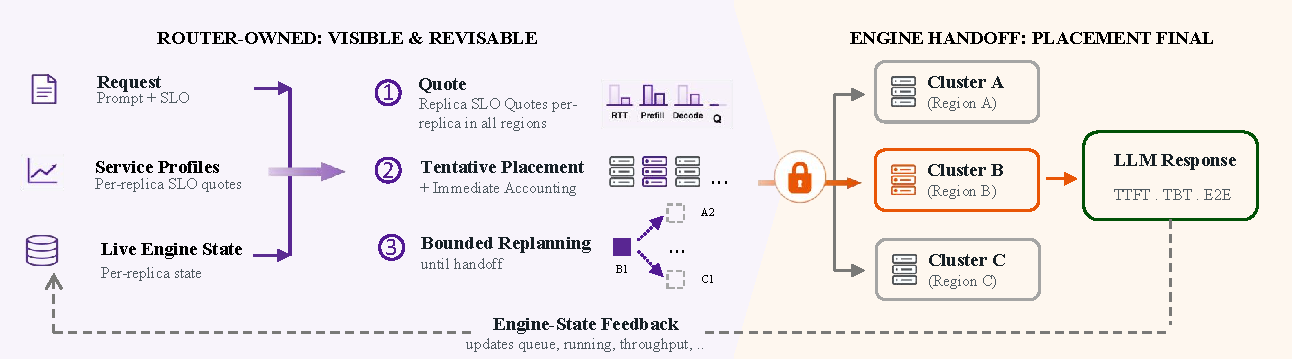
\includegraphics[width=\columnwidth]{figures/system.pdf}
    \caption{
    \textbf{RAVEL request lifecycle and ownership boundary.}
    On arrival, RAVEL constructs replica-specific SLO quotes, selects a
    tentative placement, and immediately accounts the request's prospective
    demand.
    While Router-owned, the request remains eligible for bounded reassignment,
    with tentative ownership and prospective accounting transferred together.
    Capacity-gated dispatch initiates engine handoff; only successful handoff
    makes placement final.
    Live engine state feeds back into subsequent quotes and accounting.
    }
    \label{fig:ravel-overview}
\end{figure}


\subsection{Overview}
\label{sec:design:overview}

RAVEL realizes the separation exposed by
Figure~\ref{fig:motivation}: arrival establishes demand visibility, Router
ownership preserves placement revisability, and successful engine handoff
establishes finality.
While Router-owned, each request has exactly one tentative replica owner and
one prospective demand representation.
Its destination may change as new demand or serving-state feedback arrives,
but its demand remains visible throughout.
After successful handoff, the serving engine owns the request and its
geographic placement is no longer revised.

Figure~\ref{fig:ravel-overview} summarizes this lifecycle.
On arrival, RAVEL constructs request-specific SLO quotes for candidate
replicas, chooses an initial virtual placement, and immediately accounts the
request's prospective demand at that replica.
Subsequent arrivals and engine feedback may trigger bounded replanning over a
cohort of still-Router-owned requests.
A reassignment moves both tentative ownership and replica-dependent
prospective demand to the new replica.
Requests approach execution through a shallow capacity-gated dispatch
frontier; a rejected handoff restores Router ownership, whereas a successful
handoff transfers ownership to the serving engine and makes placement final.

The design maintains three classes of invariants.
\emph{Single representation:} each Router-owned request has exactly one
tentative owner and one prospective demand representation.
\emph{Bounded mobility:} only Router-owned requests may move, and replanning is
causal and bounded in both time and scope.
\emph{Explicit finality:} tentative placement, hold expiration, and dispatch
eligibility do not commit a request; only successful engine handoff does.
The following sections describe how RAVEL enforces these properties.


\subsection{Replica SLO Quotes}
\label{sec:design:feasibility}

Revisability is useful only if the Router can determine which replicas remain
SLO-feasible for each request.
Because regional capacity is request-dependent
(Section~\ref{sec:problem:feasibility}), RAVEL represents each candidate using
a request- and replica-specific SLO quote rather than a request-independent
load score.
A quote summarizes whether the request is predicted to satisfy its applicable
SLOs, the request-specific objective used to rank viable targets, and
secondary capacity-pressure information.

Let $c\in\mathcal{C}$ denote a serving cluster,
$\mathcal{R}_c$ its replicas, $c(r)$ the cluster containing replica $r$, and
$\mathcal{R}=\bigcup_c\mathcal{R}_c$.
For request $i$ and candidate replica $r$, RAVEL constructs
\begin{equation}
    Q_{i,r}(t)
    =
    \left(
        \Phi_{i,r}(t),
        \widehat{T}^{\mathrm{obj}}_{i,r}(t),
        \mathbf{z}_{i,r}(t)
    \right),
    \label{eq:ravel-quote}
\end{equation}
where $\Phi_{i,r}(t)$ indicates whether all applicable SLO constraints are
predicted to hold,
$\widehat{T}^{\mathrm{obj}}_{i,r}(t)$ is the request-class-specific objective
used for ordering and slack calculations, and
$\mathbf{z}_{i,r}(t)$ contains secondary capacity-pressure signals.
Quotes use only information causally available at time $t$ and are online
predictions rather than formal SLO guarantees.

RAVEL combines calibrated cluster-level service profiles with live and
prospective replica state.
At active Decode concurrency $n$, it models Prefill service for prompt size
$p$ as
$P_{c,n}(p)=b_{c,n}+a_{c,n}p$ and uses $d_c(n)$ for calibrated
post-first-token Decode time per token.
For request $i$ and replica $r$, let
$\widehat{S}^{\mathrm{pre}}_{i,r}$ denote predicted Prefill-side service delay,
including live engine Prefill debt, Router-owned prompt work ahead of $i$, the
request's own prompt demand, and tentative assignments made earlier in the
same planning pass.
RAVEL predicts
\begin{equation}
    \widehat{\mathrm{TTFT}}_{i,r}(t)
    =
    (t-a_i)
    +
    \rho_{o_i,c(r)}
    +
    \widehat{S}^{\mathrm{pre}}_{i,r},
    \label{eq:ravel-ttft}
\end{equation}
where $a_i$ is request arrival time and
$\rho_{o_i,c(r)}$ is directed WAN delay from origin $o_i$ to cluster $c(r)$.
The elapsed term directly charges time already spent under Router ownership,
so a previously feasible replica may become infeasible as request slack
shrinks.

RAVEL evaluates each SLO according to its semantics rather than collapsing
them into one latency score.
For LATENCY requests, TTFT and TBT feasibility are checked independently:
a lower predicted TTFT cannot compensate for a predicted TBT violation.
For completion-oriented requests, RAVEL separates a conservative
output-demand estimate used for feasibility from an expected estimate used
for shared service-pressure accounting, avoiding both optimistic admission
and systematic over-accounting.
Appendix~\ref{sec:appendix:quotes} gives the complete TTFT, TBT, and completion
equations, calibration procedure, runtime sources, and fallback rules.


\subsection{Immediate and Transferable Demand Accounting}
\label{sec:design:accounting}

Figure~\ref{fig:motivation} shows that placement revisability loses much of its
value when already-arrived work is withheld from capacity accounting.
RAVEL therefore makes tentative demand visible immediately and exactly once,
without making its placement final.
Every Router-owned request is associated with one tentative replica queue and
one set of replica-dependent prospective charges.

When request $i$ receives a virtual placement at replica $r$, it immediately
enters $r$'s Router-owned queue.
Its prompt contributes to the queue-ahead Prefill work observed by later
quotes, including quotes constructed later in the same planning pass.
The Router also maintains lightweight prospective completion-service and
LATENCY/TBT pressure signals.
These signals complement, rather than replace, the replica's live pending and
running engine state.

Replanning must preserve this visibility as placement changes.
If $i$ moves from replica $r$ to $r'$, RAVEL atomically transfers its tentative
queue ownership and recomputes the replica-dependent prospective charges for
$r'$.
The serialized control path ensures that a planning snapshot observes
request $i$ at exactly one tentative owner---never at both replicas and never
at neither.
The destination then exposes the transferred demand to all subsequent quote
and placement decisions.

Visibility also remains continuous across the ownership boundary.
Successful handoff ends Router queue ownership, after which committed work is
represented by live engine state and an active-service charge until terminal
completion.
A rejected handoff restores the Router-owned prospective state.
These transitions establish RAVEL's central accounting invariant:
\emph{tentative work is immediately visible, but visibility does not make its
placement final}.
Appendix~\ref{sec:appendix:accounting} gives exact charge definitions, transfer
operations, deduplication rules, lifecycle transitions, and stale-callback
protection.


\subsection{Bounded Pre-Handoff Replanning}
\label{sec:design:replanning}

Later arrivals can expose stale allocations, but exploiting them requires
revisability to remain bounded in both time and scope.
RAVEL therefore reconsiders only Router-owned requests whose placements can
still change.
Committed work remains fixed but continues to affect later quotes through live
engine state.
Planning is event-driven, serialized, and coalesced so that each pass operates
on a consistent prospective view.

\paragraph{Bounding the revisable interval.}
For selected non-LATENCY requests, RAVEL preserves a short observation window
before dispatch.
Importantly, the request is already tentatively placed and prospectively
accounted during this interval; the hold changes only how long the placement
remains revisable.

Let
\[
\sigma_i^{\mathrm{arr}}
=
\max\!\left\{
0,\,
\Delta_i-
\min_r\widehat{T}^{\mathrm{obj}}_{i,r}(a_i)
\right\}
\]
denote the request's arrival-time planning slack, where $\Delta_i$ is its
applicable TTFT or completion planning budget.
RAVEL sets
\begin{equation}
    h_i
    =
    \begin{cases}
        \min\!\left\{
            \rho_i^{\min},
            \sigma_i^{\mathrm{arr}}
        \right\},
        & \text{if $i$ is hold-eligible},\\
        0,
        & \text{otherwise},
    \end{cases}
    \label{eq:ravel-mobility-hold}
\end{equation}
where $\rho_i^{\min}$ is the minimum positive RTT to a remote serving cluster.
Thus, deliberate observation is bounded by both a network timescale and the
request's available planning slack.
LATENCY requests use $h_i=0$.
Expiration of $h_i$ makes the request dispatch-eligible; it neither removes
its prospective accounting nor commits its placement.

\paragraph{Bounding replanning scope.}
Each planning pass considers a deterministic deadline-first prefix of at most
$K$ movable requests.
Requests outside the cohort retain their tentative owners and enter the
planning snapshot as fixed context.
Within the cohort, each selected placement immediately updates pass-local
prospective state before the next request is evaluated.
With $R=|\mathcal{R}|$ candidate replicas and effective cohort bound
$K_{\mathrm{eff}}$, one greedy pass performs
$O(K_{\mathrm{eff}}R)$ request--replica quote comparisons.
Under sustained completion pressure, RAVEL may expand the effective cohort
within the deployment's finite sequence capacity; this changes how much
Router-owned work is reconsidered, not the placement or commitment semantics.

\paragraph{Choosing initial and revised placements.}
RAVEL uses the same SLO-aware placement rule for an arrival and for requests
reconsidered during replanning.
If at least one replica is predicted feasible, the Router selects among
feasible targets.
If none is feasible, it first minimizes normalized predicted SLO violation.
Remaining choices are ordered lexicographically by
\emph{SLO safety}, \emph{capacity pressure}, and finally
\emph{efficiency and stability}.
The capacity-pressure tier discourages broadly substitutable requests from
occupying scarce SLO-feasible capacity, while lower-priority signals include
predicted service cost, movement, prefix locality, and deterministic
tie-breaking.
Consequently, locality or stability cannot override an avoidable predicted
SLO miss.

Replanning applies this same rule to the bounded movable cohort.
After each target is selected, RAVEL immediately updates pass-local
prospective state so that later requests in the same pass observe the demand
created by earlier tentative choices.
Algorithm~\ref{alg:ravel-control} summarizes the resulting Router control loop.
Appendix~\ref{sec:appendix:replanning} and
Appendix~\ref{sec:appendix:placement-key} provide the exact trigger predicates,
eligibility rules, cohort ordering, reassignment limits, and placement key.


\begin{algorithm}[t]
\caption{\textsc{RAVEL} Router Control Loop}
\label{alg:ravel-control}
\small

\Fn{\textnormal{\textsc{OnArrival}}($i$)}{
    $Q_i \gets \textsc{QuoteReplicas}(i)$\;
    $r_i \gets \textsc{SLOAwarePlace}(i,Q_i)$\;
    \textsc{AssignAndAccount}($i,r_i$)\;
    \tcp{Visible immediately; placement remains tentative}

    $h_i \gets \textsc{MobilityHold}(i,Q_i)$\;
    \If{$h_i = 0$}{
        \textsc{RequestReplan}()\;
    }
    \Else{
        \textsc{ArmReplan}($h_i$)\;
    }
}

\BlankLine

\Fn{\textnormal{\textsc{Replan}}()}{
    $C \gets \textsc{BoundedMovableCohort}()$\;
    \tcp{Only Router-owned requests are movable}

    \For{$i \in C$}{
        $Q_i \gets \textsc{QuoteReplicas}(i)$\;
        $r_i' \gets \textsc{SLOAwarePlace}(i,Q_i)$\;
        \textsc{TransferOrRefresh}($i,r_i'$)\;
        \tcp{Update prospective state before the next request}
    }
}

\BlankLine

\Fn{\textnormal{\textsc{Dispatch}}($i$)}{
    \If{\textsc{Held}($i$) \textbf{or} \textsc{FrontierBlocks}($i$)}{
        \Return\;
    }

    $r_i \gets \textsc{TentativeOwner}(i)$\;
    $s \gets \textsc{AttemptHandoff}(i,r_i)$\;

    \If{$s=\textsc{Rejected}$}{
        \textsc{RestoreRouterOwnership}($i,r_i$)\;
    }
    \ElseIf{$s=\textsc{Committed}$}{
        \textsc{FinalizePlacement}($i,r_i$)\;
        \tcp{Successful handoff is the commitment boundary}
    }
}
\end{algorithm}


\subsection{Commitment and Execution Protection}
\label{sec:design:commitment}

Revisability must end at a precise boundary, and execution after that boundary
must preserve the assumptions under which the placement was judged feasible.
RAVEL therefore separates approaching commitment, committing ownership, and
protecting execution after handoff.

\paragraph{Capacity-gated dispatch.}
A shallow dispatch frontier limits how much Router-owned work approaches
commitment at once.
The frontier determines \emph{when} a tentatively placed request may be handed
to its engine; it does not choose \emph{where} the request executes.
Work behind the frontier remains tentatively placed, prospectively accounted,
and eligible for replanning.
A request becomes dispatch-eligible when its tentative replica has sufficient
engine headroom, bounding proximity to commitment without introducing a
separate placement or admission policy.
Appendix~\ref{sec:appendix:frontier} gives the frontier construction and
headroom test.

\paragraph{Engine handoff as the commitment boundary.}
Commitment is an ownership transition rather than a timer or queue event.
For a dispatch-eligible request, RAVEL attempts replica registration followed
by creation of the engine-facing posting task.
Only successful completion of the handoff transfers the request from
Router-owned, revisable state to engine-owned, final state.
Failures before this boundary restore or clean the Router-owned state; failures
after handoff terminate the committed attempt without reopening geographic
placement.
Attempt identifiers prevent stale callbacks from modifying newer ownership or
accounting state.
Thus, tentative placement, hold expiration, dispatch eligibility, and temporary
removal from a Router queue are all non-commitment events.

\paragraph{Preserving quote assumptions at the engine.}
Final placement remains useful only if local execution preserves the service
conditions under which that placement was considered feasible.
In particular, Prefill--Decode interference can invalidate a TBT-feasible
quote after handoff.
When Chunked Prefill is enabled and LATENCY Decode is active, RAVEL exports the
tightest applicable TBT requirement and deadline metadata to a local serving
adapter.
The adapter combines this requirement with a calibrated conservative Prefill
envelope to bound the next Prefill quantum and gives LATENCY requests
deadline/TBT-aware local priority, while non-LATENCY work retains stable FCFS
behavior.
This mechanism protects the execution assumptions underlying replica quotes;
it does not introduce another geographic placement decision.

Together, these mechanisms complete the lifecycle derived in
Section~\ref{sec:problem}:
\emph{arrival makes demand visible, Router ownership keeps placement revisable,
and successful engine handoff makes placement final}.
Appendix~\ref{sec:appendix:handoff} and
Appendix~\ref{sec:appendix:tbt-control} give the complete ownership state
machine, failure transitions, activation rules, and local scheduling details.
